\documentclass[a4paper]{article}
\usepackage[english]{babel}
\usepackage[utf8]{vietnam}

%\usepackage{vntex}
\usepackage{listings}%chen code
%\usepackage[english,vietnam]{babel}
%\usepackage[utf8]{inputenc}

%\usepackage[utf8]{inputenc}
%\usepackage[francais]{babel}
\usepackage{a4wide,amssymb,epsfig,latexsym,multicol,array,hhline,fancyhdr}

\usepackage{amsmath}
\usepackage{lastpage}
\usepackage[lined,boxed,commentsnumbered]{algorithm2e}
\usepackage{enumerate}
\usepackage{color}
\usepackage{graphicx}							
% Standard graphics package
\usepackage{array}
\usepackage{tabularx, caption}
\usepackage{multirow}
\usepackage{multicol}
\usepackage{rotating}
\usepackage{graphics}
\usepackage[a4paper,left=2cm,right=2cm,top=1.8cm,bottom=2.8cm]{geometry}
\usepackage{setspace}
\usepackage{epsfig}
\usepackage{tikz}
\usetikzlibrary{arrows,snakes,backgrounds}
\usepackage[unicode]{hyperref}
%can file puenc.def trong thu muc goc de option [unicode] tao ra bookmark bang tieng Viet
\hypersetup{urlcolor=blue,linkcolor=black,citecolor=black,colorlinks=true} 
%\usepackage{pstcol} 								
% PSTricks with the standard color package

\newtheorem{theorem}{{\bf Theorem}}
\newtheorem{property}{{\bf Property}}
\newtheorem{proposition}{{\bf Proposition}}
\newtheorem{corollary}[proposition]{{\bf Corollary}}
\newtheorem{lemma}[proposition]{{\bf Lemma}}


%\usepackage{fancyhdr}
\setlength{\headheight}{40pt}
\pagestyle{fancy}
\fancyhead{} % clear all header fields
\fancyhead[L]{
 \begin{tabular}{rl}
    \begin{picture}(25,15)(0,0)
    \put(0,-8){
\includegraphics[width=8mm, height=8mm]{hcmut.png}}
    %\put(0,-8){\epsfig{width=10mm,figure=hcmut.eps}}
   \end{picture}&
	%
\includegraphics[width=8mm, height=8mm]{hcmut.png} & %
	\begin{tabular}{l}
		\textbf{\bf \ttfamily Ho Chi Minh City University of Technology, VNU-HCM}\\
		\textbf{\bf \ttfamily Faculty of Computer Science \& Engineering}
	\end{tabular} 	
 \end{tabular}
}
\fancyhead[R]{
	\begin{tabular}{l}
		\tiny \bf \\
		\tiny \bf 
	\end{tabular}  }
\fancyfoot{} % clear all footer fields
\fancyfoot[L]{\scriptsize \ttfamily Assignment - Mathematical Modeling Course, 2018-2019}
\fancyfoot[R]{\scriptsize \ttfamily Page {\thepage}/\pageref{LastPage}}
\renewcommand{\headrulewidth}{0.3pt}
\renewcommand{\footrulewidth}{0.3pt}


%%%
\setcounter{secnumdepth}{4}
\setcounter{tocdepth}{3}
\makeatletter
\newcounter {subsubsubsection}[subsubsection]
\renewcommand\thesubsubsubsection{\thesubsubsection .\@alph\c@subsubsubsection}
\newcommand\subsubsubsection{\@startsection{subsubsubsection}{4}{\z@}%
                                     {-3.25ex\@plus -1ex \@minus -.2ex}%
                                     {1.5ex \@plus .2ex}%
                                     {\normalfont\normalsize\bfseries}}
\newcommand*\l@subsubsubsection{\@dottedtocline{3}{10.0em}{4.1em}}
\newcommand*{\subsubsubsectionmark}[1]{}
\makeatother


\begin{document}

\begin{titlepage}

\begin{center}
HO CHI MINH CITY UNIVERSITY OF TECHNOLOGY, VNU-HCM\\
FACULTY OF COMPUTER SCIENCE \& ENGINEERNG
\end{center}

\vspace{1cm}

\begin{figure}[h!]
\begin{center}

\includegraphics[width=3cm]{hcmut.png}
\end{center}
\end{figure}

\vspace{1cm}


\begin{center}
\begin{tabular}{c}
\multicolumn{1}{l}{\textbf{{\Large MATHEMATICAL MODELING}}}\\
~~\\
\hline
\\
\multicolumn{1}{l}{\textbf{{\Large Assignment}}}\\
\\
\textbf{\Huge Mathematical model for UTXO selection}\\
\\
\hline
\end{tabular}
\end{center}

\vspace{3cm}

\begin{table}[h]
\begin{tabular}{rrl}

\hspace{5 cm} & Tutor: Huỳnh Tường Nguyên & (htnguyen@hcmut.edu.vn)\\
& Class: HLMT1, & Group: 4\\
& Student members: & Đặng Xuân Bình - 51100277 \\
& & Lê Hoàng Bửu - 51100330 \\

\end{tabular}
\end{table}

\begin{center}
{\footnotesize Ho Chi Minh, 04/2019}
\end{center}
\end{titlepage}


%\thispagestyle{empty}
\selectlanguage{english}
\newpage
\tableofcontents
\newpage


%%%%%%%%%%%%%%%%%%%%%%%%%%%%%%%%%
\section{Introduction}

$\indent$\textcolor{red}{Write context here ...}


A decentralized cryptocurrency is a digital asset using cryptography systems collectively to secure the transactions and integrity without the third party's intervention. All the transactions in the system are registered on a ledger called blockchain that is constituted of a sequence of blocks. Each block contains an unfixed number of transactions and also a hash of the previous block so that all transactions in the blockchain are immutable and valid. A significant example of this kind cryptocurrency is Bitcoin introduced in 2008 which has currently over \$141 billion in the coin market, with an average of 229K transactions daily and around 183.89 GB of storage\footnote{https://coinmarketcap.com}.

In transaction-based blockchains, the selection strategy of UTXOs for the transaction plays an essential role in cryptocurrency balance management of any wallet. An optimized coin selection strategy should satisfy hard constraints and essential goals of three principal groups such as users, community and miners. Owing to consumers, they would like to create a transaction that minimizes the transaction fee and also reserves the privacy of their behaviors. By contrast, miners focus on mining transactions which have a higher fee as much as possible. To the community, the large UTXO pool size becomes a dramatic problem because it drops down the transaction processing performance and also produces a high cost of memory consumption. Like Bitcoin system, a snapshot of the current state required additional space in the memory to store objects for processing transactions \cite{Chepurnoy:2018}.

In this work, we consider problem of strategy research in order to select a set of UTXOs for a given transaction which should cost a minimum fee for miners or gather as much as possible small UTXO in order to reduce the UTXO pool size. 
The remainder of this report is organized in the following. Section \ref{formul} presents short context and requirement of the considering problem. Then, we present our work in Section \ref{model}. Section \ref{eval} summaries the performance evaluation and discussion on experimental results. Finally, we conclude our work in the last section.

%%%%%%%%%%%%%%%%%%%%%%%%%%%%%%%%%
\section{Problem formulation}\label{fornul}

$\indent$\textcolor{red}{Describe clearly problem statement or requirement of the problem that needs to be modeled.}

%%%%%%%%%%%%%%%%%%%%%%%%%%%%%%%%%
\section{Proposed model}\label{model}

$\indent$\textcolor{red}{Variables:}


\textcolor{red}{Constraints:}


\textcolor{red}{Objective function:}

%%%%%%%%%%%%%%%%%%%%%%%%%%%%%%%%%
\section{Experimental evaluation}\label{eval}

$\indent$\textcolor{red}{Input format:}

Tập dữ liệu bao gồm 133 file data định dạng .dat tương ứng với 133 trường hợp địa chỉ chứa các UTXOs đang khảo sát. Quan sát tập dữ liệu sẽ giúp ta hiểu rõ hơn về việc các UTXOs được chọn trong mạng lưới như thế nào. Tập dữ liệu bao gồm 133 trường hợp, trong đó không có địa chỉ nào có 1 hoặc không có UTXOs; có 99 địa chỉ chứa từ 2 đến 10 UTXOs trong tổng số 133 địa chỉ, chiếm tỉ lệ cao nhất(75\%); có 19 trường hợp có từ 11 đến 100 UTXOs (chiếm khoảng 14.39\% tổng thể) và 14 trường hợp có từ 101 đến 100000 UTXOs (khoảng 10.61\% tổng thể). Figure 1 thể hiện rõ phân bố tần suất của các UTXOs trong các địa chỉ.

\newpage
\begin{center}
	\begin{figure} []
		\begin{center}
			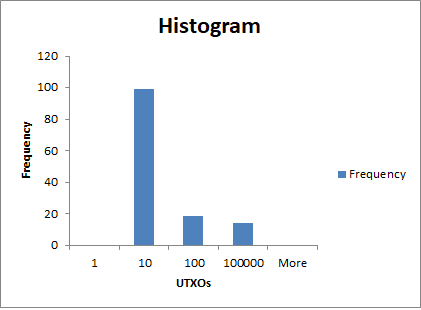
\includegraphics[scale=1]{tansuatUTXOs}
		\end{center}
		\caption{Tần suất UTXOs trong các địa chỉ}
		\label{refhinh1}
	\end{figure}
\end{center}

<Cấu trúc file "dat.dat">
\begin{lstlisting}[frame=single]

/*********************************************
* OPL 12.9.0.0 Data
* Author: Tanaka Kai
* Creation Date: May 5, 2019 at 2:39:14 PM
*********************************************/
datFiles = {"5ad448a959678302d59e6f75",
"5ad44bfdce94cf05c955f862",
"5ad44e0ece94cf05c955f864",
"5ad44e1bce94cf05c955f865",
.......
.......
.......			
"5ad4c6024c372215dd13d6bd",
"5ad4cb594c372215dd13d6be",
"5ad4cb834c372215dd13d6bf"};

\end{lstlisting}


<Cấu trúc 1 file dữ liêu "[ID].dat">
\begin{lstlisting}[frame=single]

input = <
2, 
1, 
61480, 
1048576, 
1.38313609467456, 
756, 
756, 
34, 
1352, 
330, 
0, 
0, 
>;

UTXOs = { 
<1, 148, 30234>, 
<2, 148, 33116>, 
};

output = { 
<1, 34, 61480>, 
};

\end{lstlisting}

\textcolor{red}{Output format:}

Sau khi xử lí bằng IBM CPLEX Optimization Studio 12.9.0, kết quả được đưa về dạng file csv để thuận tiện cho việc xử lý sau này.

\begin{center}
	\begin{figure} [ht]
		\begin{center}
			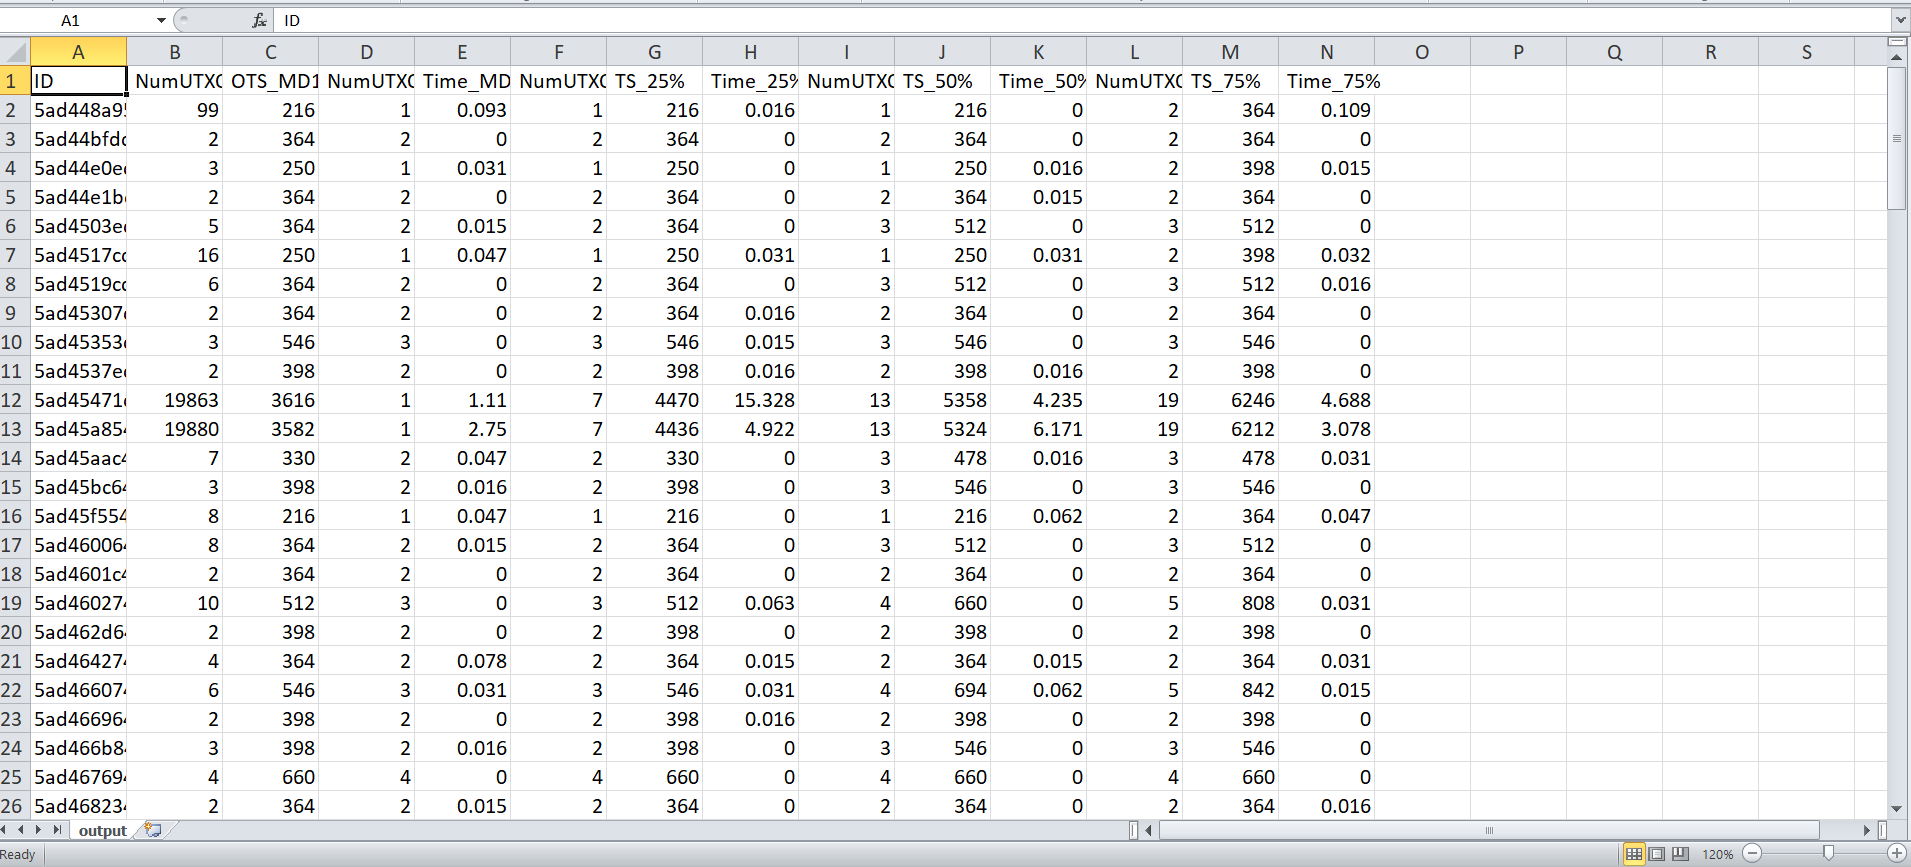
\includegraphics[scale=.43]{output}
		\end{center}
		\caption{Output format}
		\label{refhinh1}
	\end{figure}
\end{center}

\textcolor{red}{Implementation in GLPK/AMPL:} IBM CPLEX Optimization Studio 12.9.0

<File "sub.mod">
\begin{lstlisting}[frame=single]

tuple vin {
	int vid;
	int vsize;
	int vValue; 
}

tuple vout {
	int vid;
	int vsize;
	int vValue; 
}

tuple inputSet {
	int n;
	int m;
	float outValue;
	float M;
	float alpha;
	float T;
	float epsilon;
	int beta;
	int txsize;
	int iosize;
	float cout;
	float coutValue;
}

inputSet input = ...;

{vin} UTXOs = ...;

{vout} output = ...;

int outputSize = sum(e in output) e.vsize;

dvar boolean a[UTXOs];
dvar int+ zsize;
/*range n = 1..input.n;*/
//dexpr float minv=min(forall(e in UTXOs, a[e] diff 0)) a[e]*e.vsize;
dexpr int inputSize = sum(e in UTXOs) a[e]*e.vsize;
dexpr int inputValue = sum(e in UTXOs) a[e]*e.vValue;

dexpr int transactionSize = inputSize + outputSize + zsize;
dexpr float zvalue = inputValue - (input.outValue + input.alpha*transactionSize);
minimize transactionSize;

subject to {
	cons0:
	(zvalue <= input.epsilon - 0.0001) => (zsize == 0);
	(zvalue >= input.epsilon) => (zsize == input.beta);
	cons1:
	inputSize + outputSize + zsize <= input.M;
	cons2: 
	forall (out in output)
	out.vValue >= input.T;
	cons3:
	zvalue >= 0;
}

int numUTXO = sum(e in UTXOs) a[e];

execute {
	writeln(numUTXO);
}

\end{lstlisting}



<File "mainflow.mod">
\begin{lstlisting}[frame=single]

 {string} datFiles = ...;

float k = ...;

float Y = ...;

main {
	var file = new IloOplOutputFile("output.txt"); 
	file.writeln("ID, NumUTXO, OTS_MD1, NumUTXOUsed_MD1, Time_MD1, NumUTXOUsed_25%, TS_25%, Time_25%, NumUTXOUsed_50%, TS_50%, Time_50%, NumUTXOUsed_75%, TS_75%, Time_75%")
	
	var source = new IloOplModelSource("sub.mod");
	var cplex = new IloCplex();
	var def = new IloOplModelDefinition(source);
	
	for (var datFile in thisOplModel.datFiles) { 	
	
	var opl = new IloOplModel(def, cplex);
	var data = new IloOplDataSource(datFile+".dat");
	opl.addDataSource(data);
	opl.generate();
	if (cplex.solve()) {
	opl.postProcess();
	
	file.write(datFile+", ");
	file.write(opl.input.n+", ");
	file.write(cplex.getObjValue()+", ");
	file.write(opl.numUTXO+", ");
	file.write(cplex.getSolvedTime()+", ");
	
	var optValue = cplex.getObjValue();
	writeln("OBJ = "+ cplex.getObjValue());
	
	//k = 0,25
	var source2 = new IloOplModelSource("sub_2.mod");
	var cplex = new IloCplex();
	var def2 = new IloOplModelDefinition(source2);
	var opl2 = new IloOplModel(def2, cplex);
	var data2 = new IloOplDataElements();
	data2.k = 0.25;
	data2.Y = optValue;
	opl2.addDataSource(data);
	opl2.addDataSource(data2);
	
	opl2.generate();
	
	if (cplex.solve()) {
	file.write(opl2.selected+", ");
	file.write(opl2.transactionSize+", ");
	file.write(cplex.getSolvedTime()+", ");
	}
	else {
	writeln("No solution") 			
	}
	
	//k = 0.5
	var source2 = new IloOplModelSource("sub_2.mod");
	var cplex = new IloCplex();
	var def2 = new IloOplModelDefinition(source2);
	var opl2 = new IloOplModel(def2, cplex);
	var data2 = new IloOplDataElements();
	data2.k = 0.5;
	data2.Y = optValue;
	opl2.addDataSource(data);
	opl2.addDataSource(data2);
	
	opl2.generate();
	
	if (cplex.solve()) {
	file.write(opl2.selected+", ");
	file.write(opl2.transactionSize+", ");
	file.write(cplex.getSolvedTime()+", ");
	}
	else {
	writeln("No solution") 			
	}
	
	//k = 0.75
	var source2 = new IloOplModelSource("sub_2.mod");
	var cplex = new IloCplex();
	var def2 = new IloOplModelDefinition(source2);
	var opl2 = new IloOplModel(def2, cplex);
	var data2 = new IloOplDataElements();
	data2.k = 0.75;
	data2.Y = optValue;
	opl2.addDataSource(data);
	opl2.addDataSource(data2);
	
	opl2.generate();
	
	if (cplex.solve()) {
	file.write(opl2.selected+", ");
	file.write(opl2.transactionSize+", ");
	file.writeln(cplex.getSolvedTime()+", ");
	}
	else {
	writeln("No solution") 			
	}
	}	
	else {
	writeln("No solution"); 		
	}
	opl.end();
	} 
}
\end{lstlisting}



\textcolor{red}{Experimental results}

Mô hình đã đề xuất được giải bởi IBM CPLEX Studio Optimization 12.9.0. Giá trị của $\gamma$ trong Model 2 được thực nghiệm lần lượt là 25\%, 50\%, 75\%. Kết quả lấy được sẽ được so sánh với kết quả sẵn có của các phương pháp HVF, LVF, OF.

\begin{table}[ht]
	\begin{tabular}{|l|l|l|l|l|l|l|l|}
		\hline
		Method     & HVF    & LVF     & OF     & Model 1 & Model 2($\gamma$=25\%) & Model 2($\gamma$=50\%) & Model 2($\gamma$=75\%) \\ \hline
		NoSelected & 330.00 & 1361.00 & 855.00 & 315.00  & 373.00        & 469.00        & 559.00        \\ \hline
	\end{tabular}
\end{table}

\begin{center}
	\begin{figure} [ht]
		\begin{center}
			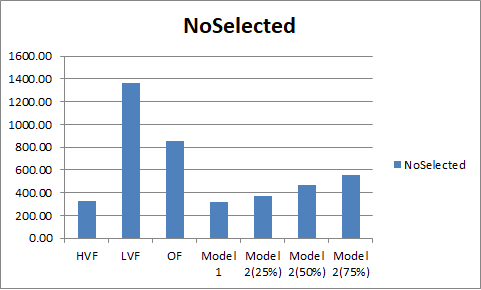
\includegraphics[scale=1]{NoSelected}
		\end{center}
		\caption{Số lượng UTXOs được chọn ở mỗi phương pháp}
		\label{refhinh1}
	\end{figure}
\end{center}

Đối với Model 1, số lượng UTXOs được chọn rất ít, tổng cộng chỉ có 315 cái được chọn, thấp hơn cả mô hình HVF. Model 2 với các giá trị $\gamma$ được khảo sát cho kết quả UTXOs được chọn nhiều hơn nhưng vẫn ở mức thấp, chưa bằng mô hình OF và thấp hơn nhiều so với mô hình LVF.

\begin{table}[ht]
	\begin{tabular}{|l|l|l|l|l|l|l|l|}
		\hline
		Method  & HVF & LVF & OF & Model 1 & Model 2($\gamma$=25\%) & Model 2($\gamma$=50\%) & Model 2($\gamma$=75\%) \\ \hline
		RunTime & 69  & 79  & 62 & 13.234  & 74.622        & 81.703        & 52.393        \\ \hline
	\end{tabular}
\end{table}

\begin{center}
	\begin{figure} [ht]
		\begin{center}
			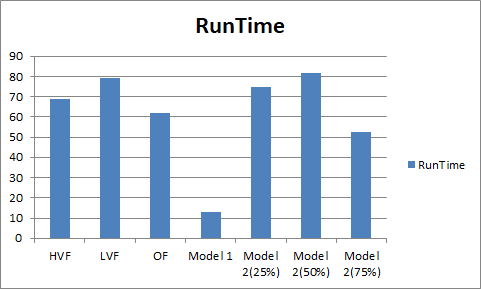
\includegraphics[scale=1]{RunTime}
		\end{center}
		\caption{Thời gian chạy giải thuật của mỗi phương pháp}
		\label{refhinh1}
	\end{figure}
\end{center}

Từ những số liệu thống kê trên, ta có thể thấy Model 1 tốn rất ít thời gian sô với các mô hình còn lại( chỉ xấp xỉ 13.234s). Trong khi đó, Model 2 cho kết quả thời gian chạy khá tương đồng với các mô hình HVF, LVF, OF.

\begin{table}[ht]
	\begin{tabular}{|l|l|l|l|l|l|l|l|}
		\hline
		Method  & HVF & LVF & OF & Model 1 & Model 2($\gamma$=25\%) & Model 2($\gamma$=50\%) & Model 2($\gamma$=75\%) \\ \hline
		TransactionSize & 399724 & 551632 & 477526 & 85618   & 93794         & 107900        & 121152        \\ \hline
	\end{tabular}
\end{table}

\begin{center}
	\begin{figure}[!ht]
		\begin{center}
			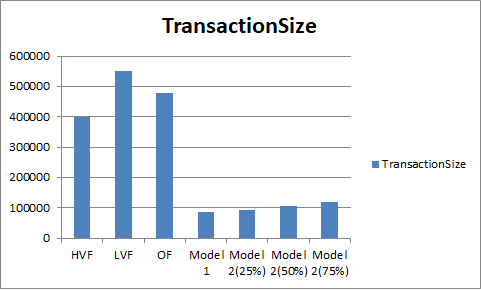
\includegraphics[scale=1]{TransactionSize}
		\end{center}
		\caption{Tổng kích thước giao dịch của mỗi phương pháp}
		\label{refhinh1}
	\end{figure}
\end{center}

Kích thước giao dịch của các Model 1 và 2 là khá nhỏ và thấp hơn nhiều so với các mô hình HVF, LVF, OF.\\

Từ những số liệu trên, ta có thể thấy mô hình 1 tuy có thời gian chạy rất thấp nhưng số lượng UTXOs được chọn cũng rất thấp. Trong khi đó, ở mô hình 2, với những giá trị $\gamma$ để kiểm soát lần lượt là 25\%, 50\%, 75\%, ta có thể thấy thời gian chạy vẫn được giữ xấp xỉ với các mô hình HVF, LVF, OF, nhưng số lượng UTXOs được chọn đã được tăng lên đáng kể, đồng thời kích thước giao dịch vẫn tương đối ổn định so với mô hình 1.

%%%%%%%%%%%%%%%%%%%%%%%%%%%%%%%%%
\newpage
\section{Conclusion}
$\indent$
Trong bài báo cáo này, nhóm chúng em đã hiện thực hai mô hình đã đưa ra để đánh giá về việc giải quyết hai mục tiêu thiết yếu khi tạo giao dịch mới trên blockchain.đó là giảm thiếu kích thước giao dịch để có phí giao dịch tối thiểu và thu nhỏ tập UTXO. mô hình 1 tối thiểu được kích thước giao dịch tuy nhiên không giải quyết được nhu cầu thu nhỏ tập UTXO nên chúng ta đưa ra mô hình 2 để giải quyết được cả 2 vấn đề này. Mô hình 2 được đưa ra để vừa có thể chọn được càng nhiều UTXO càng tốt nhưng không làm cho kích thước giao dịch quá lớn, do chúng ta đã kiểm soát bằng tỉ lệ gamma nên luôn đảm bảo kích thước giao dịch không lớn quá mức cho phép làm tăng phí giao dịch. Qua đó ta có thể thấy được so với các mô hình hiện tại là HVF và LVF thì rõ ràng mô hình trên hiệu quả hơn. Mặc dù cần được thử nghiệm với các tập dữ liệu lớn hơn nữa  nhưng rõ ràng mô hình đã đưa ra hoàn toàn khả thi để đưa vào thực tế.

\newpage
%%%%%%%%%%%%%%%%%%%%%%%%%%%%%%%%%

\begin{thebibliography}{80}


\bibitem{http://wikipedia:2015} wikipedia.
``\textbf{link: http://en.wikipedia.org/}'',
\textit{}, last access: 05/05/2015.


	\bibitem{Frey2016}	Frey, D., Makkes, M. X., Roman, P.-L., Taiani,  F.,  Voulgaris, S.: Bringing secure Bitcoin transactions to your smartphone. The 15th International Workshop on Adaptive and Reflective Middleware, (2016).
	
	\bibitem{Andreas2014} Antonopoulos, A. M.: Mastering Bitcoin. 2nd edn. O'Reilly Media, CA 95472 (2014).
	
	\bibitem{Bitcoinjs} Bitcoinjs: Open Source Organisation for Bitcoin JavaScript Libraries,https://github.com/bitcoinjs. Last accessed 15 August 2018.
	
	\bibitem{Bitcoinj}	Bitcoinj: Library for working with the Bitcoin protocol,https://bitcoinj.github.io. Last accessed 10 August 2018.
	
	\bibitem{Yanovich:2016} Yanovich, Y., Mischenko, P.,  Ostrovskiy,  A.:  Shared Send Untangling in Bitcoin, White paper, Bitfury Group Limited (2016).
	
	\bibitem{Patrick-Dai:2016} Dai, P., Mahi, N., Earls, J., Norta, A.: Smart-Contract Value-Transfer Protocols on a Distributed Mobile Application Platform,  https://qtum. org/uploads/files/cf6d69348ca50dd985b60425ccf282f3.pdf, (2016).
	
	\bibitem{Sergi:2017} Sergi, D.-S., Cristina, P.-S., Guillermo, N.-A., Jordi, H.-J.: Analysis of the Bitcoin UTXO set, IACR Cryptology ePrint Archive, (2017).
	
	\bibitem{Mark-Erhardt:2016} Erhardt, M.: An Evaluation of Coin Selection
	Strategies, Master thesis, Karlsruhe Institute of Technology, URL: http://murch.one/wp-content/uploads/2016/11/erhardt2016coinselection.pdf, (2016).
	
	\bibitem{Zahnentferner:2018} Zahnentferner, J.: Chimeric ledgers: Translating and unifying utxo-based and account-based cryptocurrencies, Cryptology ePrint Archive, Report 2018/262, 2018. https://epri nt. iacr. org/2018/262, (2018).
	
	\bibitem{Chepurnoy:2018} Chepurnoy, A., Kharin, V., Meshkov, D.: A Systematic Approach To Cryptocurrency Fees. IACR Cryptology ePrint Archive, (2018).
\end{thebibliography}
\end{document}

